 
\subsection{Recipes for engineering templates}
\label{ssec:recipes_technical}

\TBD It is not clear (2020-11-19) whether data from maintenance
templates need to be reduced by the pipeline. This section and the
recipes described therein serves as a placeholder and may be removed
later.

%------------------------------------------------------------------------------------------------------------------
\subsubsection{Pupil imaging}\label{rec:metis_pupil_imaging}
\label{sssec:pupil_imaging}

\TBD This recipe refers to pupil imaging using the science
detectors. Presumably it only contains the most basic reduction
steps. There may have to be separate recipes for the various
subsystems.

\begin{recipedef}
  Name                 & \hyperref[rec:metis_pupil_imaging]{\REC{metis_pupil_imaging}}                     \\
  Purpose:             & Apply basic reduction to pupil imaging data.  \\
  Requirements:        & --                                            \\
  Type:                & Maintenance                                   \\
  Templates:           & \TPL{METIS_pup_lm}                            \\
                       & \TPL{METIS_pup_n}                             \\
  Input data:          & \hyperref[dataitem:lm_pupil_raw]{\RAW{LM_PUPIL_RAW}} or \hyperref[dataitem:n_pupil_raw]{\RAW{N_PUPIL_RAW}} \\
  Matched keywords:    & Detector ID                                   \\
  Algorithm            & \TBD                                          \\
  Output data:         & \hyperref[dataitem:lm_pupil_reduced]{\PROD{LM_PUPIL_REDUCED}} or \hyperref[dataitem:n_pupil_reduced]{\PROD{N_PUPIL_REDUCED}} \\
  Expected accuracies: & None                                          \\
  QC1 parameters:      & None                                          \\
\end{recipedef}

\clearpage
%------------------------------------------------------------------------------------------------------------------
\subsubsection{Chopper Home Position recipe \REC{metis_img_chophome}}\label{ssec:metisimgchophome}
The recipe \hyperref[rec:metis_img_chophome]{\REC{metis_img_chophome}} aims to detect undefined chopper mirror zero positions after switching on the chopper (e.g. after instrument interventions) or induced by unforeseen events like earthquakes (cf. Section "Chopper Home Position" in  \cite{METIS-calibration_plan}).
\begin{figure}[ht]
  \centering
  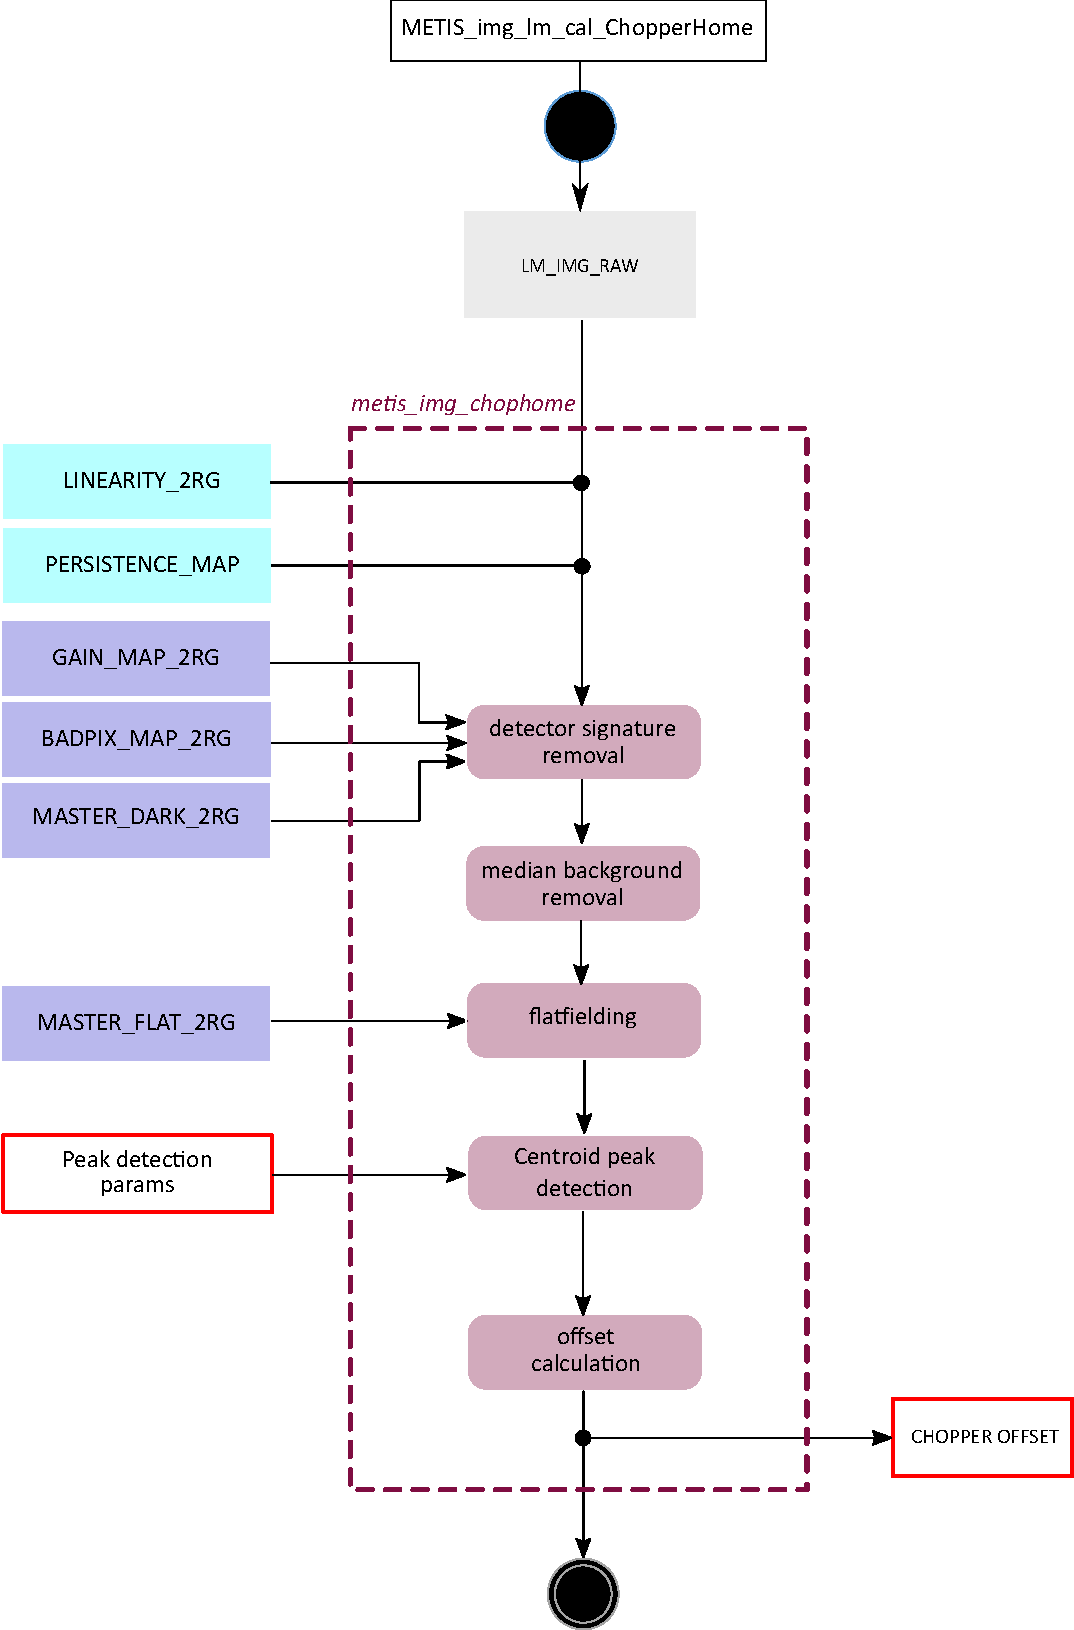
\includegraphics[width=0.5\textheight]{figures/metis_img_chophome_v0.83.pdf}
  \caption[Recipe: \REC{metis_img_chophome}]{\REC{metis_img_chophome} --
    Recipe workflow to detect the zero position of the chopper mirror.}
  \label{Fig:rec_chop_home}
\end{figure}

\begin{recipedef}\label{rec:metisimgchophome}\label{rec:metis_img_chophome}
Name:		& \hyperref[rec:metis_img_chophome]{\REC{metis_img_chophome}} \\
Purpose:	& Detection of the chopper mirror home position \\
Type:		& Calibration\\
Requirements: & TBD \\
Templates:      & \TPL{METIS_img_lm_cal_ChopperHome} \\
Input data:     & \hyperref[dataitem:lm_chopperhom_raw]{\RAW{LM_CHOPPERHOME_RAW}} \\
                & \hyperref[dataitem:persistence_map]{\EXTCALIB{PERSISTENCE_MAP}}  \\
                & \hyperref[dataitem:linearity_2rg]{\STATCALIB{LINEARITY_2RG}}  \\
                & \hyperref[dataitem:gain_map_2rg]{\PROD{GAIN_MAP_2RG}}  \\
                & \hyperref[dataitem:badpix_map_2rg]{\PROD{BADPIX_MAP_2RG}}  \\
                & \hyperref[dataitem:master_dark_2rg]{\PROD{MASTER_DARK_2RG}}  \\
                & \hyperref[dataitem:master_img_flat_lm]{\PROD{MASTER_IMG_FLAT_LM}}  \\
Parameters: 	& TBD\\
Algorithm:      & remove detector signature\\
                & remove median background\\
                & apply flatfield\\
                & detect reference source from \ac{WCU} via centroid peak detection\\
                & Calculate mirror offset\\
Output data:	& Offset of the chopper mirror to be piped either into the \ac{ICS} for correction \\
                & or to be used in thee pipeline for astrometric correction\\
Expected accuracies: & 0.1mas accuracy of the centroid position (cf. \cite{METIS-calibration_plan})\\
QC1 parameters: & \QC{TBD}: TBD\\
\end{recipedef}
\clearpage

%------------------------------------------------------------------------------------------------------------------
% Moved to https://github.com/AstarVienna/METIS_DRLD/issues/101
% \subsubsection{Plate-scale calibration}
% \TODO{Plate-scale calibration}

%------------------------------------------------------------------------------------------------------------------
\subsubsection{Fringing correction}
\label{rec:metis_fringing_correction}

It is unclear for the time being how much of a problem will be with the METIS
detectors, and what the best strategy will be to tackle it. Therefore, the
method to use will be chosen based on AIT results (\REQ{METIS-9151}, for rationale and basic method description see Ch.~3.12 in the Calibration Plan \cite{METIS-calibration_plan}).

Whether a stand-alone recipe will be required, or if the fringe-map will become
part of another recipe, is part of that uncertainty. If needed, the design of
said recipe will be minimal work and is thus omitted in this document.

%------------------------------------------------------------------------------------------------------------------
\subsubsection{Calibration of slit losses}\label{sssec:adc_slitlosses}
The recipes \hyperref[rec:metis_lm_adc_slitloss]{\REC{metis_lm_adc_slitloss}} (Fig.~\ref{Fig:rec_lm_adc_slitloss}) and \hyperref[rec:metis_n_adc_slitloss]{\REC{metis_n_adc_slitloss}} (Fig.~\ref{Fig:rec_n_adc_slitloss}) aims to determine the slitlosses induced by the fixed positions of the \ac{ADC} (cf. Section "Calibration of slit losses" in  \cite{METIS-calibration_plan})). This recipe is to be carried out once in a while and creates the slitlosses to be included in the static calibration database.
\begin{figure}[ht]
  \centering
  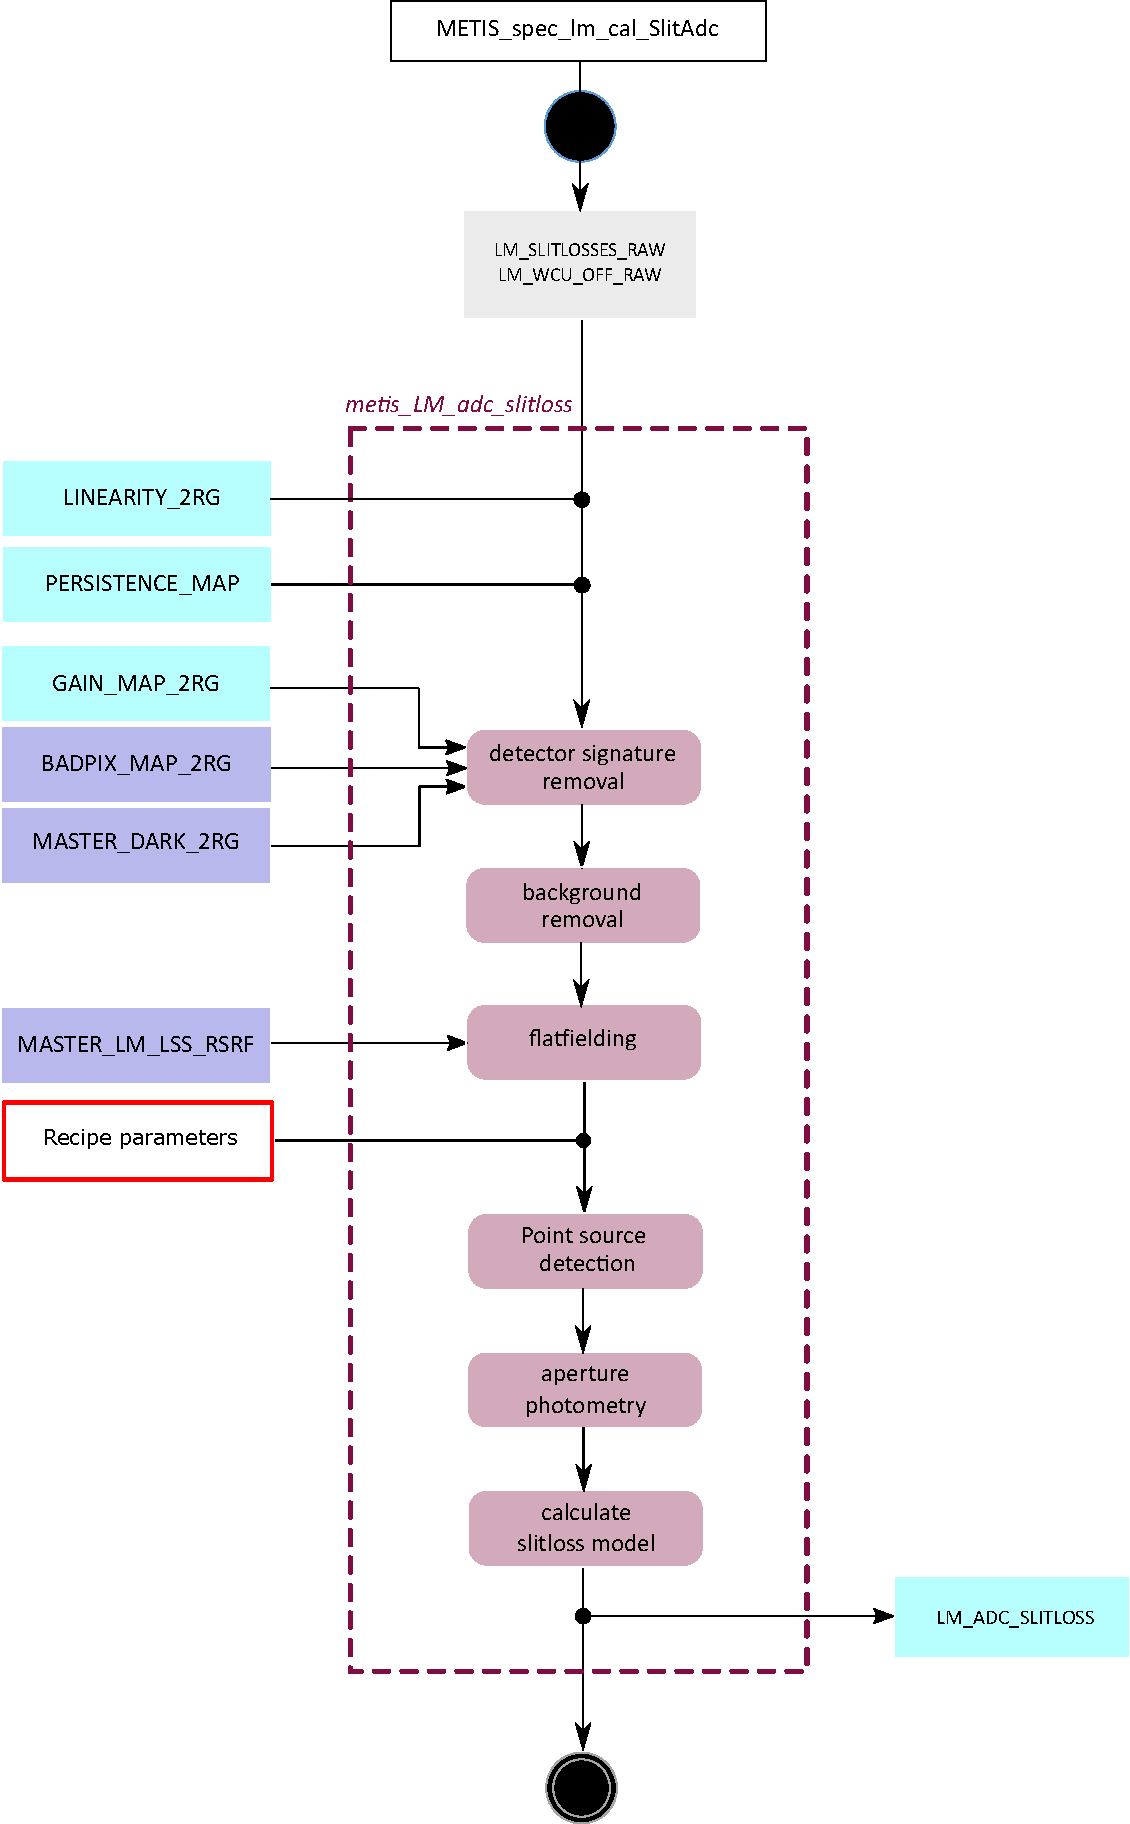
\includegraphics[width=0.5\textheight]{figures/metis_lm_lss_adc_slitloss_v0.83.pdf}
  \caption[Recipe: \REC{metis_lm_adc_slitloss}]{\REC{metis_lm_adc_slitloss} --
    Recipe workflow to determine the \ac{ADC} induced slit losses.}
  \label{Fig:rec_lm_adc_slitloss}
\end{figure}

\begin{recipedef}\label{rec:metislmadcmslitloss}\label{rec:metis_lm_adc_slitloss}
Name:		& \hyperref[rec:metis_lm_adc_slitloss]{\REC{metis_lm_adc_slitloss}} \\
Purpose:	& Determination of the \ac{ADC} induced slit losses \\
Type:		& Calibration\\
Requirements: &  METIS-6074, METIS-2757, METIS-9099\\
Templates:           & \TPL{METIS_spec_lm_cal_SlitAdc} \\
Input data:     & \hyperref[dataitem:lm_slitlosses_raw]{\RAW{LM_SLITLOSSES_RAW}} \\
                & \hyperref[dataitem:lm_wcu_off_raw]{\RAW{LM_WCU_OFF_RAW}} \\
                & \hyperref[dataitem:persistence_map]{\EXTCALIB{PERSISTENCE_MAP}}  \\
                & \hyperref[dataitem:linearity_2rg]{\STATCALIB{LINEARITY_2RG}}  \\
                & \hyperref[dataitem:gain_map_2rg]{\PROD{GAIN_MAP_2RG}}  \\
                & \hyperref[dataitem:badpix_map_2rg]{\PROD{BADPIX_MAP_2RG}}  \\
                & \hyperref[dataitem:master_dark_2rg]{\PROD{MASTER_DARK_2RG}}  \\
                & \hyperref[dataitem:master_img_flat_lm]{\PROD{MASTER_IMG_FLAT_LM}}  \\
%Parameters: 	& TBD\\
Algorithm:      & remove detector signature\\
                & remove dark\\
                & apply flatfield\\
                & detect reference source from \ac{WCU} via centroid peak detection\\
                & apply aperture photometry\\
                & calculate (simple) slitloss model (details to be defined)\\
Output data:	& \hyperref[dataitem:lm_adc_slitloss]{\STATCALIB{LM_ADC_SLITLOSS}} (Slit loss model as function of the wavelength and object position across the slit \\
Expected accuracies: & 3\% (cf. \cite{METIS_calerrbudget})\\
QC1 parameters: & \QC{TBD}: TBD\\
\end{recipedef}


\begin{figure}[ht]
  \centering
  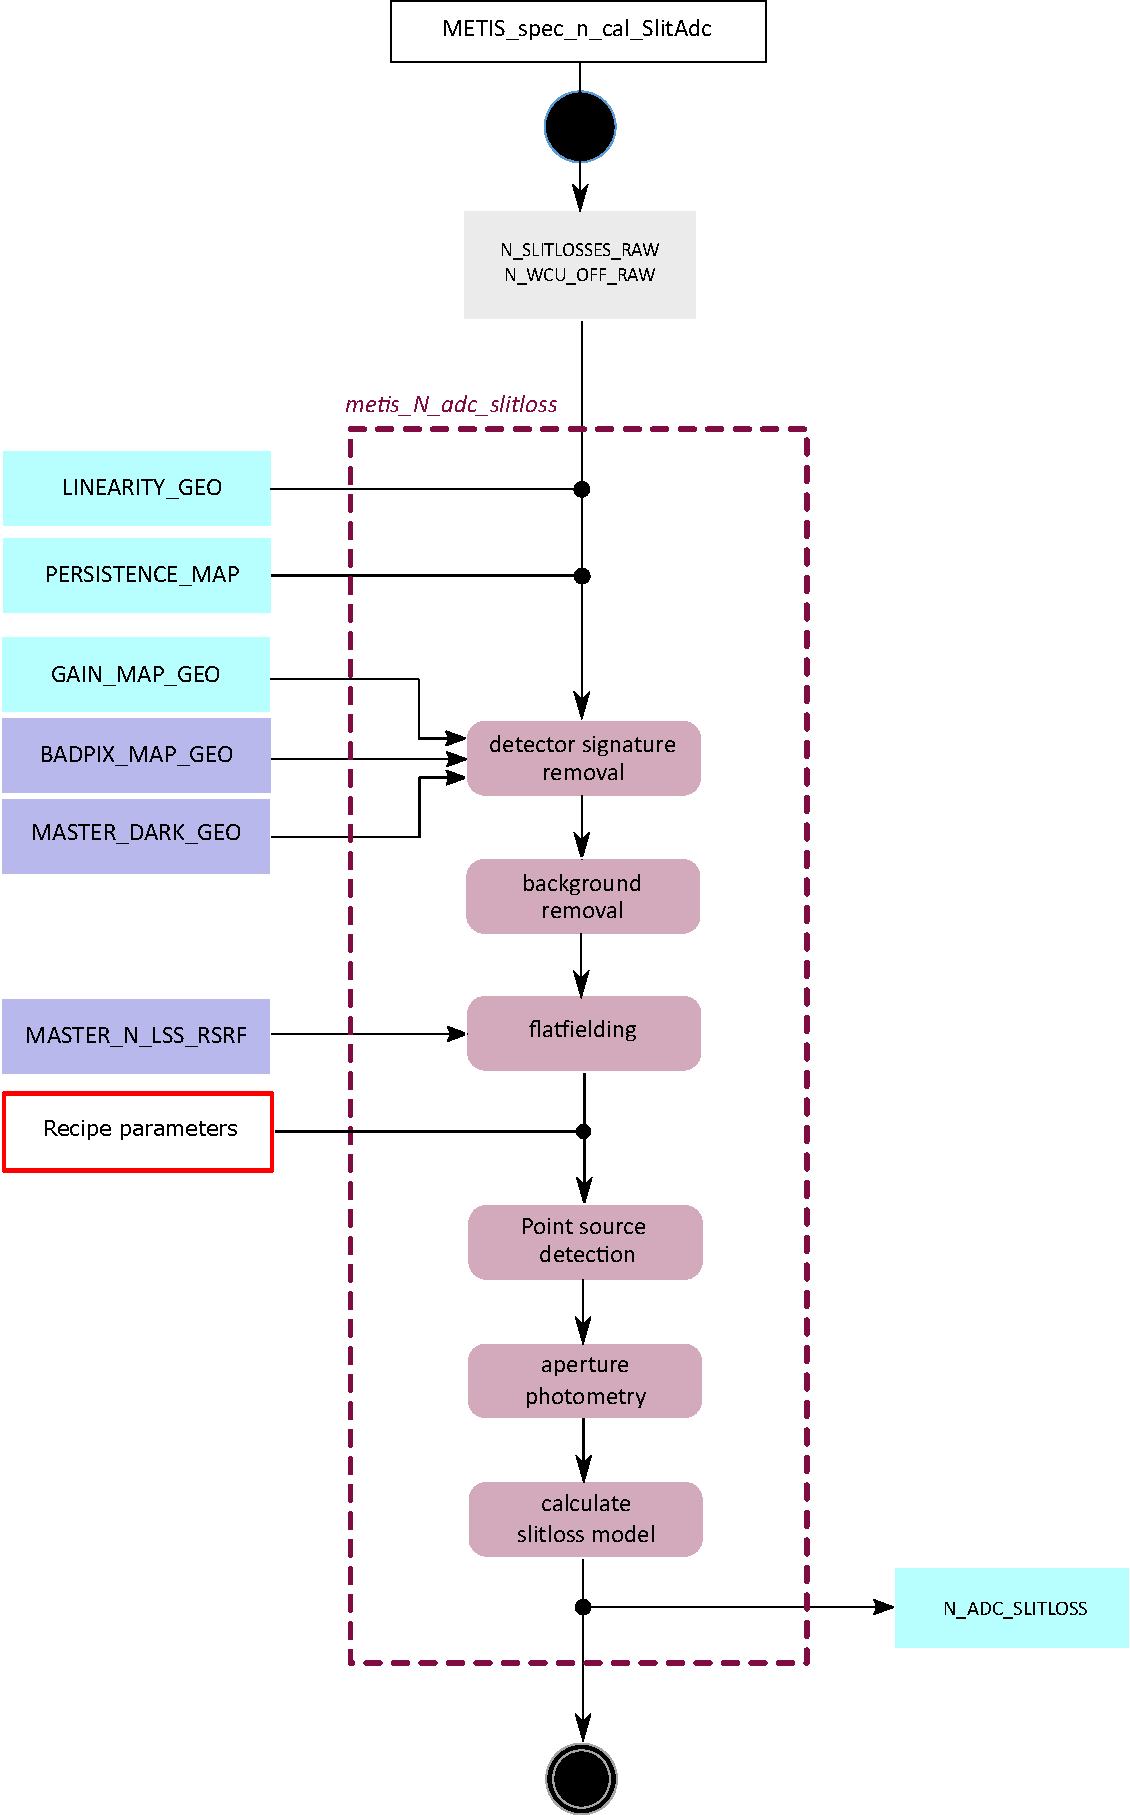
\includegraphics[width=0.5\textheight]{figures/metis_n_lss_adc_slitloss_v0.83.pdf}
  \caption[Recipe: \REC{metis_n_adc_slitloss}]{\REC{metis_n_adc_slitloss} --
    Recipe workflow to determine the \ac{ADC} induced slit losses.}
  \label{Fig:rec_n_adc_slitloss}
\end{figure}

\begin{recipedef}\label{rec:metisnadcmslitloss}\label{rec:metis_n_adc_slitloss}
Name:		& \hyperref[rec:metis_n_adc_slitloss]{\REC{metis_n_adc_slitloss}} \\
Purpose:	& Determination of the \ac{ADC} induced slit losses \\
Type:		& Calibration\\
Requirements: & METIS-6074, METIS-2757, METIS-9099 \\
Input data:     & \hyperref[dataitem:n_slitlosses_raw]{\RAW{N_SLITLOSSES_RAW}} \\
                & \hyperref[dataitem:n_wcu_off_raw]{\RAW{N_WCU_OFF_RAW}} \\
                & \hyperref[dataitem:persistence_map]{\EXTCALIB{PERSISTENCE_MAP}}  \\
                & \hyperref[dataitem:linearity_geo]{\STATCALIB{LINEARITY_GEO}}  \\
                & \hyperref[dataitem:gain_map_geo]{\PROD{GAIN_MAP_GEO}}  \\
                & \hyperref[dataitem:badpix_map_geo]{\PROD{BADPIX_MAP_GEO}}  \\
                & \hyperref[dataitem:master_dark_geo]{\PROD{MASTER_DARK_GEO}}  \\
                & \hyperref[dataitem:master_img_flat_n]{\PROD{MASTER_IMG_FLAT_N}}  \\
%Parameters: 	& TBD\\
Algorithm:      & remove detector signature\\
                & remove dark\\
                & apply flatfield\\
                & detect reference source from \ac{WCU} via centroid peak detection\\
                & apply aperture photometry\\
                & calculate (simple) slitloss model (details to be defined)\\
Output data:	& \hyperref[dataitem:n_adc_slitloss]{\STATCALIB{N_ADC_SLITLOSS}} (Slit loss model as function of the wavelength and object position across the slit) \\
Expected accuracies: & 3\% (cf. \cite{METIS_calerrbudget})\\\\
QC1 parameters: & \QC{TBD}: TBD\\
\end{recipedef}


%%% Local Variables:
%%% mode: latex
%%% TeX-master: "METIS_DRLD"
%%% End:
